\documentclass[12pt, a4paper]{article}

\usepackage[fleqn]{amsmath}
\usepackage[margin = 1in]{geometry}

\setlength{\parskip}{\medskipamount}
\setlength{\parindent}{0pt}
\renewcommand{\baselinestretch}{1.2}

\usepackage{graphicx}
\graphicspath{ {/} }

\usepackage{multicol}
%\usepackage{wrapfig}

\usepackage[
backend=bibtex,
style=authoryear,
citestyle=authoryear
]{biblatex}
\addbibresource{refs/refs.bib}

\begin{document}
	
	\title{MultiBiDAF - A Multi-Sentence Reading Comprehension Model}
	\author{Eitan-Hai Mashiah and Noam Barda}
	\maketitle
	
	\begin{multicols}{2}
		
		\section{Introduction}
		
			Machine comprehension is a task of natural language processing wherein the algorithm is presented with a context paragraph and a query, and must answer the query using the data in the paragraph. While this is one of the classical tasks of NLP (\cite{Mccarthy1976}), interest in it has surged in recent years thanks to algorithmic advances (such as recurrent neural networks) and new benchmark datasets such as CNN/daily mail (\cite{Hermann2015}), SQuAD (\cite{Rajpurkar2016}), NewsQA (\cite{Trischler2016}) and multiRC (\cite{N18-1023}).
			
			Despite its rising popularity, performance in this task remains challenging, and algorithms' capabilities are often below those of young children (\cite{Clark2016}).
			
		\section{Datasets}
		
			We will use two datasets in this project: SQuAD for pre-training and multi-RC as the actual challenge. Both will now be described.
			
			SQuAD, the Standford Question Answering Dataset (\cite{Rajpurkar2016}) was released in 2016. It is a large dataset with over 100,000 questions written by crowd-sourced workers on wikipedia articles.
			
			It has several defining characteristics:
			\begin{enumerate}
				\item A single context paragraph has several questions attached to it.
				\item An answer is always a span of text in the paragraph. This is critical.
				\item There isn't a predetermined list of answers to choose from.
			\end{enumerate}
		
			Version 2.0 of this dataset (\cite{Rajpurkar2018}) also adds questions for which no answer exists in the paragraph, requiring the answering algorithm to also know when to abstain from answering.
			
			Currently, human performance on SQuAD (F1 = 89.452) far surpasses best machine performance (F1 = 74.422), leaving a wide gap for researchers to fill.
			
			multiRC (\cite{N18-1023}) is a fairly recent addition to machine comprehension datasets. It consists of \char`~ 6000 questions on \char`~ 800 paragraphs from 7 different knowledge domains.
			
			It's defining characteristics are:
			\begin{enumerate}
				\item Several answers are proposed for each question.
				\item Of which one or more can be true.
				\item Answering requires reasoning over several sentences (specifically, 2-4) in the paragraph that are not a single span. This is the defining characteristic of this dataset.
			\end{enumerate}
		
			The dependence on several sentences was created to force the algorithm to better "understand" the context paragraph, and thus allow better generalization.
			
			Again, we see that human performance (F1 = 86.4) is significantly better than existing algorithms (F1 = 66.1), leaving a wide gap to be addressed.
			
		\section{Baseline Model}
		
			Our attempt at improving performance on the multiRC dataset will use an existing model as the baseline, altering it in ways that should improve its performance when applied to multiRC. The model we chose for this task is the Bidirectional Attention Flow for Machine Comprehension (BIDAF) model (\cite{Seo2016}). We'll begin by describing the model at large, and will then focus on its main novelty, which is as the name suggests, its attention mechanism. See figure 1 for the complete model diagram as originally published.
			
			The layer-wise structure of the BIDAF model is:
			\begin{itemize}
				\item Character-level embedding using a character-level convolutional neural network.
				\item Word embedding layer using pre-trained word embeddings (GLoVe).
				\item A standard bi-directional multilevel LSTM dubbed the contextual embedding layer.
				\item The bi-directional attention layer, to be described in the next paragraph.
				\item Another standard bi-directional multilevel LSTM dubbed the modeling layer.
				\item An output layer with two parts: One for predicting the start token and one for predicting the end token.
			\end{itemize}
		
			More accurately, the first two layers are input to the third layer, which is then input to the attention layer. This entire process, up to the attention layer, is executed separately for the context and the query. The output of the attention layer together with the unattended output from the contextual layer are both passed to the modeling layer, and that is used to predict the outputs.
			
			The novel part of this model is the attention layer. Generally speaking, classic attention mechanisms (\cite{Bahdanau2014}):
			\begin{itemize}
				\item Summarize the entire context paragraph into a single dense vector by weighting the hidden representations of the RNN.
				\item Are dynamic, allowing the attention weights learned in a previous time step to affect the current time step.
				\item Are uni-directional, with the query attending the paragraph.
			\end{itemize}
		
			In the BIDAF model, on the other hand, the attention mechanism:
			\begin{itemize}
				\item Calculates attention for each time step and passes it on to the next layer, preventing early summarization.
				\item Is static, now allowing the attention weights from the previous time-step to affect the current time-step.
				\item Is bi-directional, from context to query and from query to context.
			\end{itemize}
		
			More concretely, the attention mechanism utilizes a T (context length) by J (query length) learnable similary matrix between the context and query words, whereby for each attending (context or query) word, the attended words are weighted using a softmax function based on the corresponding row or column of the similarity matrix, and then summed.
			
			This model has been shown to achieve state-of-the-art results on multiple datasets, including SQuAD and CNN/DailyMail.
			
			The specific implementation we'll use is the one in the allennlp project (\cite{Gardner2017ADS}). Allennlp is an open source NLP research library based on pytorch.
		
		\section{Our Model and Training Process}
		
			While the above-described output layer is a good fit for a dataset such as SQuAD, in which the answer is always a single span from the context paragraph, it is not fitting for multiRC, in which 2-4 sentences participate in the answer.
			
			To handle this setting, we replaced the original output layer by a new output layer with the following changes:
			\begin{itemize}
				\item Instead of predicting one start token and one end token, it predicts up to 4 start token. Predicting the end tokens is unnecessary, as they are by definition the end of the sentences.
				\item We changed the loss function to be the negative log probabilities of the correct start tokens.
				\item We changed the accuracy metric used for validation during training to be the proportion of correct sentences predicted. This was averaged across the entire dataset.
			\end{itemize}
		
			As the number of questions in the multiRC is clearly not sufficient to properly train a complete neural network, even with pretrained word embeddings, we opted for a two-stage process.
			\begin{enumerate}
				\item In the first stage, the model will be pre-trained on the SQuAD dataset.
				\item In the second stage, the model will be fine-tuned on the multiRC dataset.
			\end{enumerate}

			Performance will of course be evaluated on the multiRC dataset, success on which is our main concern in this project.
			
			Additionally, identifying the pertinent sentences is not sufficient to decide which answers are right. Those answers must be chosen based on their agreement with the sentences. To do so we opted for a similarity test between the relevant sentences and the answers. More specifically, we used cosine similarity between TF-IDF weighted word counts in the sentences and the answers. The weighting was of course trained on the training data.
			
			Actual training will be done a Nvidia Tesla P100 GPU on google cloud.
			
		\section{Results}
		
			Pre-training on the squad dataset was carried for 20 epochs, with best-epoch performance of @@@. See figure 2 for a complete learning curve.
			
			Training on the multiRC dataset was carried for 20 epochs, with eventual best-epoch validation performance of @@@. See figure 3 for a complete learning curve.
			
			As the multiRC test set is not publicly available, test (as opposed to validation) results can only be had by sending the model's results to the dataset authors. This process takes a few weeks, and test results were not available in time for submission.
			
		\section{Conclusion}
		
			Our validation results of @@@ are close/superior (@@@) to the state-of-the-art result of @@@.
		
			In this project we illustrated that a neural network model, utilizing a bi-directional attention flow mechanism, can achieve state-of-the-art performance on the multiRC dataset. To achieve this, the model has to undergo a modification of the output layer and subsequent fine-tuning.
			
			Future directions of research could involve either similar changes to the output layer (e.g. perhaps a NER type layer, tagging spans as belonging to the answer), or changes to the actual network.
		
	\end{multicols}

	\begin{figure*}
		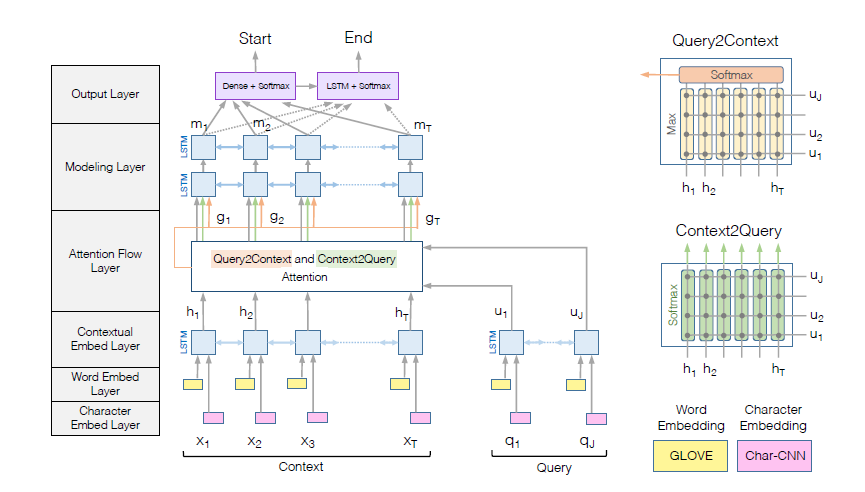
\includegraphics[width=\textwidth,height=10cm]{images/bidaf.png}
		\caption{BIDAF Model Structure}
	\end{figure*}
	
	\begin{figure*}
		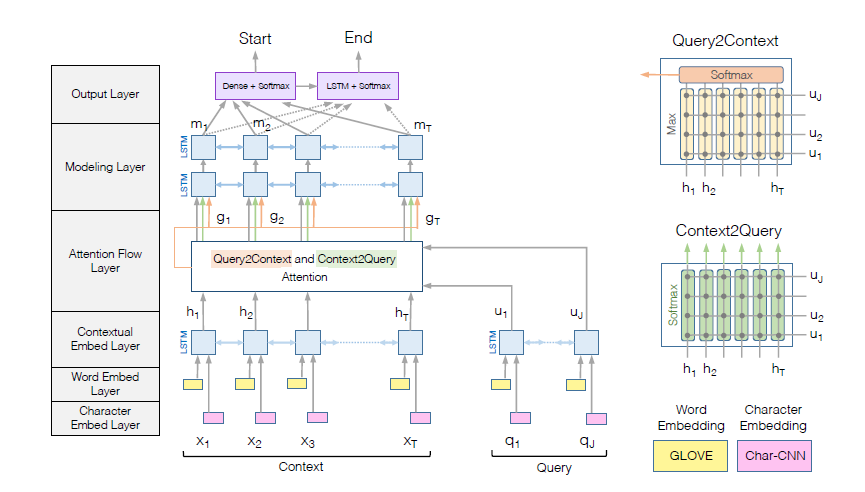
\includegraphics[width=\textwidth,height=10cm]{images/bidaf.png}
		\caption{SQuAD Pre-training Learning Curve}
	\end{figure*}
	
	\begin{figure*}
		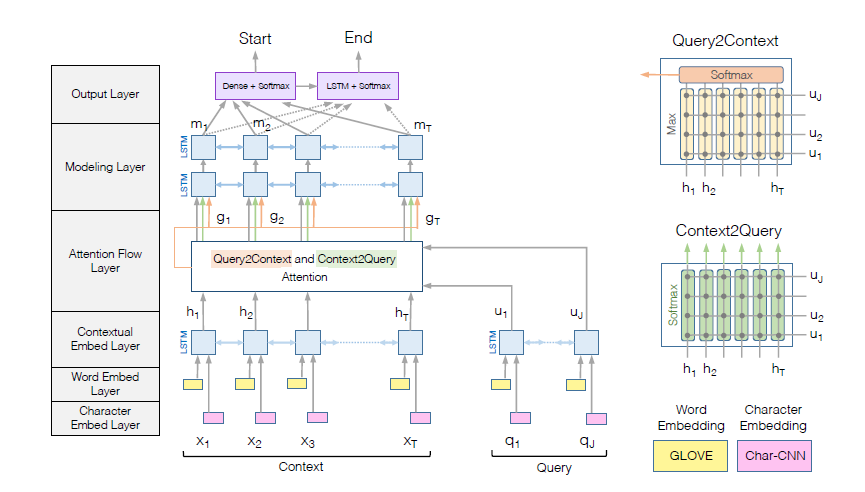
\includegraphics[width=\textwidth,height=10cm]{images/bidaf.png}
		\caption{multiRC training Learning Curve}
	\end{figure*}

	\printbibliography

%	\begin{figure}[h]
	%	\centering
	%	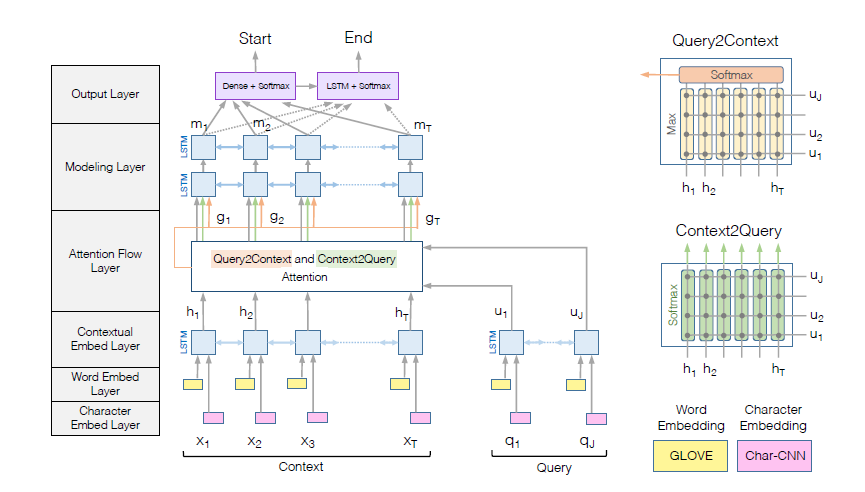
\includegraphics[width=\textwidth]{images/bidaf.png}
	%	\caption{BIDAF Model Structure}
%	\end{figure}
	
\end{document}